\section{Final Comparison}
\label{sec:comparison}
\subsection{Accuracy}
Figure~\ref{fig:final_accuracy} compares all four validation-selected
checkpoints. Both pretrained models outperform the custom networks on this
test set. For Model B, the question is whether that improvement justifies
the additional storage and computation for the intended device.
\begin{figure}[H]\centering
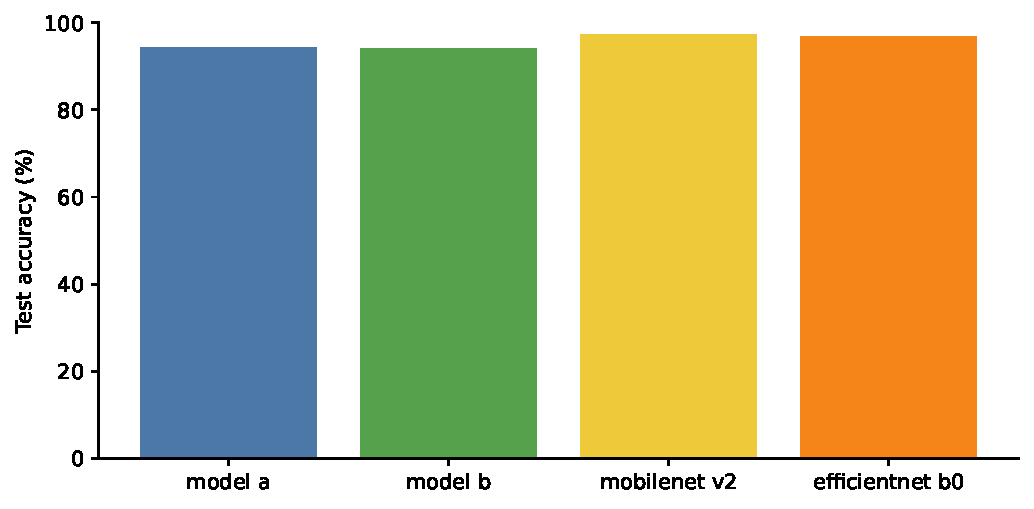
\includegraphics[width=0.96\textwidth]{figures/final_accuracy.pdf}
\caption{Held-out test accuracy using validation-selected checkpoints.}
\label{fig:final_accuracy}
\end{figure}
Relative to MobileNetV2, Model B gives \MobileAccuracyGap{} percentage points
lower test accuracy; relative to EfficientNet-B0, the difference is
\EfficientAccuracyGap{} percentage points. These are observed accuracy costs
under the tested configurations.
\subsection{Parameter Count}
The parameter totals count learned tensors only, while trainable totals reflect
the active training stage. Frozen pretraining parameters still occupy storage.
Tables~\ref{tab:custom_resources} and~\ref{tab:pretrained_resources} show
\BParams{} parameters for Model B, compared with \MobileParams{} for
MobileNetV2 and \EfficientParams{} for EfficientNet-B0. Model B saves
\MobileParamSaving\% and \EfficientParamSaving\%, respectively. Freezing
feature weights reduces the trainable count but does not remove their storage
or inference cost.
\subsection{Memory Footprint}
Figure~\ref{fig:final_resources} separates parameter count from serialized
size. Model B occupies \BSizeMiB{} MiB, compared with \MobileSizeMiB{} MiB
for MobileNetV2 and \EfficientSizeMiB{} MiB for EfficientNet-B0. These are
reductions of \MobileStorageSaving\% and \EfficientStorageSaving\%.
Serialization and buffers explain why byte reductions differ from parameter
reductions.
\begin{figure}[H]\centering
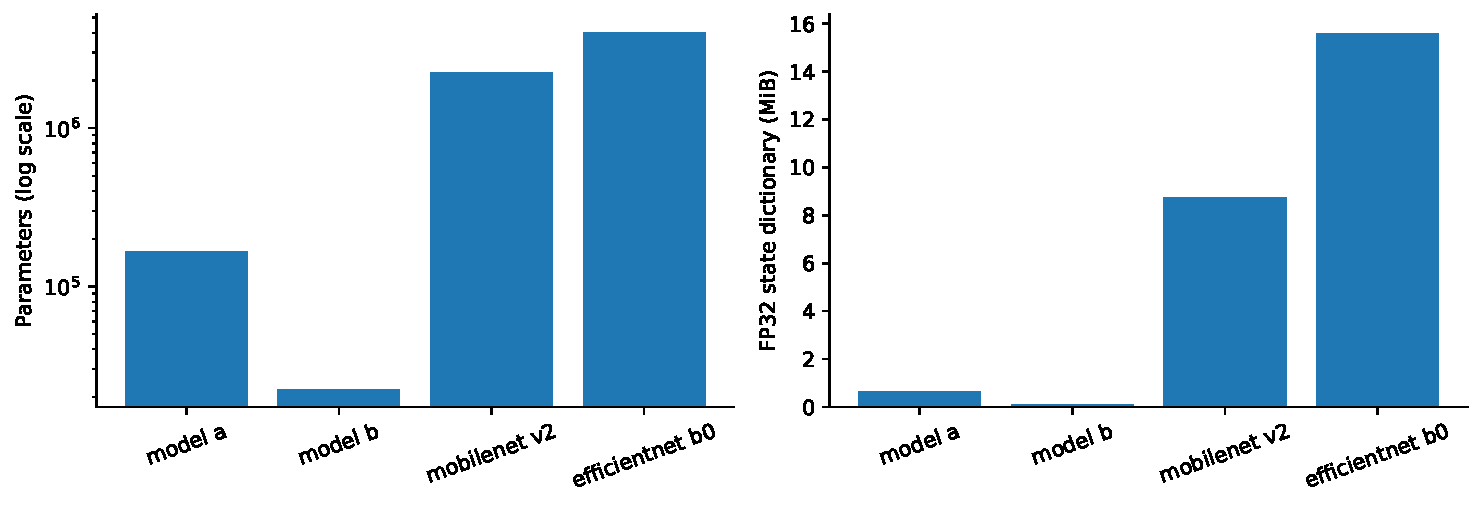
\includegraphics[width=0.96\textwidth]{figures/final_resources.pdf}
\caption{Parameter counts and measured FP32 state-dictionary sizes.}
\label{fig:final_resources}
\end{figure}

Sizes include batch-normalization buffers and serialization overhead but exclude
optimizer state. KiB and MiB use powers of 1024. The CSV column suffixes
\texttt{kb/mb} use these binary units. Disk size is not peak inference RAM;
activation and workspace memory are not measured.
\subsection{Computational Cost}
Table~\ref{tab:compute} compares one-image arithmetic counts with measured
CPU latency. Model B uses \MobileMacSaving\% fewer counted MACs than
MobileNetV2 and \EfficientMacSaving\% fewer than EfficientNet-B0. These
savings concern Conv2d and Linear operations only.
% Generated from saved experiment evidence; do not edit values.
\begin{table}[H]\centering\small
\caption{One 64x64 image: Conv/Linear arithmetic estimates and batch-one host CPU latency.}\label{tab:compute}
\begin{tabular}{lrrrr}
\toprule
Model & MACs (M) & 2xMAC (MFLOP) & CPU mean (ms) & CPU p95 (ms) \\ \midrule
Model A & 30.967 & 61.934 & 1.358 & 1.802 \\
Model B & 6.188 & 12.377 & 1.723 & 2.459 \\
MobileNetV2 & 24.461 & 48.923 & 8.452 & 13.143 \\
EfficientNet-B0 & 31.979 & 63.959 & 12.454 & 27.092 \\
\bottomrule
\end{tabular}
\end{table}


MAC accounting uses forward hooks to obtain executed layer output shapes,
kernel sizes and group counts, avoiding an external profiling dependency.
It excludes normalization, activations, pooling, residual additions and data
movement; twice MACs is only an arithmetic FLOP estimate. CPU timing uses the
Intel Core i7-13620H host, four PyTorch threads, FP32, batch one, 20 warm-ups
and 100 timed forwards. It excludes preprocessing and file I/O.
The preallocated benchmark input is a zero tensor of the required shape;
this is a forward-pass microbenchmark, not end-to-end application latency.
GPU epoch times and CPU inference times measure different workloads.
In Table~\ref{tab:compute}, Model B takes \BLatency{} ms on average versus
\ALatency{} ms for Model A despite its lower MAC count. MobileNetV2 and
EfficientNet-B0 take \MobileLatency{} ms and \EfficientLatency{} ms,
respectively.
\subsection{Edge Deployment Trade-offs}
Model B is a reasonable candidate when weight storage is the main constraint
and its accuracy cost is acceptable. Model A remains competitive when the
target resembles the measured host and latency matters more than checkpoint
size: it is faster here and has slightly higher test accuracy. MobileNetV2
is the stronger pretrained candidate in these experiments because it combines
higher accuracy with lower storage and host latency than EfficientNet-B0.
This conclusion is limited to the current split and schedule.

The pretrained models require more time per epoch, especially after unfreezing
(Table~\ref{tab:transfer_stages}). Their shorter fine-tuning schedules do not
include the original ImageNet training cost. Neither MAC counts nor host
measurements establish performance on an edge accelerator. Target-device
operator support, quantization, peak RAM, latency and power should be checked
before deployment. The present evidence establishes storage and arithmetic
savings, not energy savings.
